\subsection{Resultados da busca de revis\~ao}\label{subesec:resul da revisão}


%Nesta seção serão apresentados os resultados da pesquisa utilizando algum software, a fim de estipular o melhor uso de cada banco de dados utilizado durante o trabalho. Assim, pode-se começar com a análise no \textit{software VOSviewer}. 
%
%\begin{figure}[htp!]
	\centering
	\caption{Palavras-chave mais populares na Scopus.}
	\label{fig:scopus-09-08}
	\includegraphics[width=0.9\linewidth]{Revisao/Figuras/"scopus 09-08"}
	
	\vspace{0.2cm}
	Fonte: Elaboração própria a partir de dados da Scopus (2016 a 2022)
\end{figure}
%Na figura \ref{fig:scopus-09-08} há uma lista das palavras mais usadas como sinônimos da palavra \textit{time series analysis} ou juntas no corpo do texto dos artigos.
%A análise da base de dados no scopus foi feita na ferramenta que mostra as palavras-chave que podem ser relacionadas em cada campo de busca, com isto tem uma visão ampla do que pode ter correlação com as palavras-chave mãe da busca.
%
%Na relação entre as palavras-chave neste primeiro momento, foi obtido um resultado de 3484 palavras-chave, 212 atingindo o limite, lembrando que as palavras base a partir das quais se deve chegar ao texto \textit{``time series forecasting and time series analysis''} em Scopus.
%
%
%
%\begin{figure}[htpb!]
	\centering
	\caption{Palavras-chave mais populares na Web of Science}
	\label{fig:web-09-08}
	\includegraphics[width=0.8\linewidth]{Revisao/Figuras/"web 09-08"}
	
	
	
	\fonte{Elaboração própria a partir de dados da Web of Science (2016 a 2022)}
\end{figure}
%
%
%Na Figura \ref{fig:web-09-08} a análise do banco de dados Web of Science foi feita na ferramenta que mostra as palavras-chave que estão relacionadas em cada campo de busca, com isto você pode ter uma visão ampla do que tem correlação com as palavras-chave mãe da busca.
%
%Na relação entre as palavras-chave neste primeiro momento, teve um resultado de 305 palavras-chave, 13 atingem o limite, lembrando que as palavras base para o resultado foi \textit{``time series forecasting and time series analysis''} na web of science.
%
%O único banco de dados que não será mostrado aqui é o banco de dados Lente, porque é um excelente banco de dados e ainda não retornou muito na busca que foi feita. O site do lens retornou apenas 11 artigos com os filtros aplicados. Na \ref{etp:rev-1} é observado o campo de busca que foi usado nesta busca que deu apenas 11 artigos.





%---------------------------


Nesta seção, serão apresentados os resultados da pesquisa, utilizando um software para melhor aproveitamento de cada banco de dados utilizado no trabalho. Inicialmente, foi realizada uma análise no software VOSviewer.

\begin{figure}[htp!]
	\centering
	\caption{Palavras-chave mais populares na Scopus.}
	\label{fig:scopus-09-08}
	\includegraphics[width=0.9\linewidth]{Revisao/Figuras/"scopus 09-08"}
	
	\vspace{0.2cm}
	Fonte: Elaboração própria a partir de dados da Scopus (2016 a 2022)
\end{figure}

A Figura \ref{fig:scopus-09-08} mostra uma lista das palavras mais frequentemente utilizadas como sinônimos ou em conjunto com \textit{time series analysis} nos artigos. A análise da base de dados do Scopus foi feita com uma ferramenta que exibe as palavras-chave relacionadas em cada campo de busca, proporcionando uma visão abrangente das correlações com as palavras-chave principais.

Nesse primeiro momento, foram obtidas 3.484 palavras-chave, sendo que 212 delas atingiram o limite estabelecido. É importante destacar que as palavras-chave base utilizadas foram \textit{``time series forecasting and time series analysis''} no Scopus.

\begin{figure}[htpb!]
	\centering
	\caption{Palavras-chave mais populares na Web of Science}
	\label{fig:web-09-08}
	\includegraphics[width=0.8\linewidth]{Revisao/Figuras/"web 09-08"}
	
	
	
	\fonte{Elaboração própria a partir de dados da Web of Science (2016 a 2022)}
\end{figure}

A análise do banco de dados Web of Science, apresentada na Figura \ref{fig:web-09-08}, também foi realizada por meio de uma ferramenta que mostra as palavras-chave relacionadas em cada campo de busca. Mais uma vez, é possível obter uma visão ampla das correlações com as palavras-chave principais.

Nesse primeiro momento, foram obtidas 305 palavras-chave, sendo que 13 delas atingiram o limite estabelecido. É importante ressaltar que as palavras-chave base utilizadas foram \textit{``time series forecasting and time series analysis''} na Web of Science.

O banco de dados Lens não será apresentado aqui, pois, embora seja uma excelente fonte, não retornou muitos resultados na pesquisa realizada. O site do Lens retornou apenas 11 artigos com os filtros aplicados. Na \ref{etp:rev-1} apresenta o campo de busca utilizado nessa pesquisa, resultando nos 11 artigos encontrados.


\begin{table}[htpb!]
	\caption{Cruzamento de palavras-chave através da aplicação de filtros de ano e de linguagem}\label{tb1}
	\centering
	\begin{tabular}{@{}cp{2cm}p{1cm}p{2cm}p{1cm}p{2cm}p{2cm}p{2cm}@{}}
		\toprule
		Bases                             & \multicolumn{5}{c}{Palavras Chaves}                                                         & Resultado \\ \midrule
		\multirow{2}{*}{Scopus}           & time   series forecasting & AND & time   series analysis    &     &                         & 490       \\
		& nonlinear forecasting     & AND & time   series forecasting &     &                         & 8         \\
		\multirow{2}{*}{Web   of Science} & time   series forecasting & AND & time   series analysis    &     &                         & 126       \\
		& nonlinear forecasting     & AND & time   series forecasting &     &                         & 14        \\
		Lens                              & time   series forecasting & AND & time   series analysis    & AND & nonlinear   forecasting & 11        \\
		\multicolumn{6}{c}{Total}                                                                                                       & 649       \\ \bottomrule
	\end{tabular}
	
	\fonte{Elaboração própria a partir de dados da Scopus, Lens e Web of Science (2016 a 2022)}
\end{table}


A Tabela \ref{tb1} apresenta as palavras-chave utilizadas em cada base de dados, juntamente com o número de artigos encontrados inicialmente. No entanto, é importante ressaltar que esses dados ainda não foram processados para remover duplicatas. Após a utilização do \textit{software Mendeley} para eliminar as duplicações, restaram 308 artigos únicos, os quais serão considerados nesta revisão.




\begin{figure}[htp!]
	\centering
	\caption{Analise das quantidades de artigos em relação aos anos.}
	\label{fig:regressao-linear-dos-artigos-baseados-nos-anos}
	\includegraphics[width=0.9\linewidth]{Revisao/Figuras/"regressão linear dos artigos baseados nos anos"}
	
	\fonte{Elaboração própria a partir de dados da SANEPAR (2018 a 2020)}
\end{figure}

%A figura \ref{fig:regressao-linear-dos-artigos-baseados-nos-anos} tem com abcissas e ordenadas anos e artigos, assim a relação entre a data de publicação dos artigos ao longo do tempo.
%
%Um número considerável de artigos para analisar na Figura \ref{fig:regressao-linear-dos-artigos-baseados-nos-anos} uma análise foi feita com base em uma regressão linear dos artigos ao longo dos anos de 2016 a 2022, nesta análise obteve a seguinte equação de regressão linear:
%
%
%\begin{eqnarray}
%	y(x)&=&8,3571x - 16803 \qquad \text{Com } R^2=0,3062\label{eq1}
%\end{eqnarray}
%
%Com $y(x)$ a equação da reta na equação \eqref{eq1}. $8,3571$ é o coeficiente angular do gráfico de $ y(x)$, $16,803$ é o coeficiente linear, ou o ponto de intersecção com o eixo $y$, $x$ é a variável independente.
%
%Este coeficiente indica a proporção da variância da variável dependente que pode ser atribuída estatisticamente ao conhecimento de uma ou mais variáveis independentes \citeonline{coeficiente}. 
%
%O coeficiente de determinação mede a relação que existe entre a variável dependente e as variáveis independentes, indicando que porcentagem da variação explicada pela regressão representa da variação total. Quando:
%
%$R^2=1$: todos os pontos observados estão exatamente na reta de regressão (ajuste perfeito), ou seja, as variações de $y$ são de $100\%$ explicadas pela variação de $x_n$ através da função especificada, sem desvios em torno da função estimada. 
%
%$R^2=0$: conclui-se que as variações de $y$ são exclusivamente aleatórias e a introdução das variáveis $x_n$ no modelo não incorporará nenhuma informação sobre as variações de $y$.
%
%\begin{equation}
%	R^{2}=\frac{\left(\sum X . Y-\frac{\sum X \cdot \sum Y}{n}\right)^{2}}{\left[\sum X^{2}-\frac{\left(\sum X\right)^{2}}{n}\right] \cdot\left[\sum Y^{2}-\frac{\left(\sum Y\right)^{2}}{n}\right]}=(r)^{2}\label{eq2}
%\end{equation}
%
%Na equação \eqref{eq2} $X,Y$ é dado pelas coordenadas no plano cartesiano como por exemplo o par encomendado $(x,y)$. 
%Na equação \eqref{eq1} observa-se que obteve o $R^2=30\%$ isto implica que a linha de regressão será influenciada pelo $R^2$ que foi encontrado.
%
%Embora seja uma análise muito simples que foi realizada com a relação entre número de artigos e anos, ainda é uma validação muito boa para olhar para o teste F de significância que é dado o significado tem que ser sempre $F<5\%$ este teste também é chamado de p-valor.
%
%Tendo estes valores, é possível analisar o significado extremo da linha de regressão e observar que 2021 foi o ano em que a maioria dos artigos foram publicados sobre este tema da séries temporais.

A Figura \ref{fig:regressao-linear-dos-artigos-baseados-nos-anos} apresenta um gráfico que ilustra a relação entre o número de artigos publicados e os anos correspondentes. Foi realizada uma análise utilizando regressão linear para examinar essa relação ao longo do tempo.

A equação de regressão linear obtida foi a seguinte:

\begin{eqnarray}
	y(x) &=& 8,3571x - 16.803 \quad \text{com } R^2 = 0,3062\label{eq1}
\end{eqnarray}

Na equação \eqref{eq1}, $y(x)$ representa a equação da reta, onde $x$ é a variável independente que corresponde aos anos. O coeficiente angular da reta é de $8,3571$, e o coeficiente linear é de $-16.803$, que indica o ponto de intersecção com o eixo y.

O coeficiente de determinação, $R^2$, é utilizado para avaliar a proporção da variação na variável dependente (número de artigos) que pode ser explicada pela variação na variável independente (anos). Nesse caso, o valor de $R^2$ foi de $0.3062$, o que indica que aproximadamente 30,62\% da variação nos números de artigos pode ser explicada pela passagem do tempo.

O coeficiente de determinação mede a relação entre a variável dependente e as variáveis independentes, representando a porcentagem da variação explicada pela regressão em relação à variação total. Quando o $R^2$ é igual a 1, todos os pontos observados estão exatamente na reta de regressão, indicando um ajuste perfeito, ou seja, todas as variações em $y$ são totalmente explicadas pela variação em $x_n$ através da função especificada, sem desvios em torno da função estimada. Por outro lado, quando o $R^2$ é igual a 0, conclui-se que as variações em $y$ são exclusivamente aleatórias e a inclusão das variáveis $x_n$ no modelo não fornece nenhuma informação sobre as variações em $y$.

A fórmula do coeficiente de determinação $R^2$ é dada pela equação:
\begin{equation}
	R^{2}=\frac{\left(\sum X . Y-\frac{\sum X \cdot \sum Y}{n}\right)^{2}}{\left[\sum X^{2}-\frac{\left(\sum X\right)^{2}}{n}\right] \cdot\left[\sum Y^{2}-\frac{\left(\sum Y\right)^{2}}{n}\right]}=(r)^{2}\label{eq2}
\end{equation}
Na equação \eqref{eq2}, $X$ e $Y$ representam as coordenadas no plano cartesiano, como por exemplo, o par ordenado $(x,y)$. Na análise realizada com a relação entre o número de artigos e os anos, obteve-se um valor de $R^2=30\%$, o que implica que a linha de regressão é influenciada pelo valor encontrado de $R^2$.

Embora seja uma análise simples da relação entre o número de artigos e os anos, essa é uma validação significativa para observar o teste F de significância, que deve ser sempre inferior a 5\%, também conhecido como valor-p. Com base nesses valores, é possível analisar o significado da linha de regressão e observar que o ano de 2021 foi o ano em que a maioria dos artigos foi publicada sobre o tema das séries temporais.

\begin{table}[H]
	\centering
	\caption{Fator de impacto}\label{tb2}
	\begin{tabular}{@{}cp{3cm}p{3cm}c@{}}
		\toprule
		Revista cientíica      & Quantidade de plubicação & Qualidade da revista & H-INDEX \\\midrule
		Neurocomputing         & 27                         & Q1                     & 143     \\
		IEEE Access            & 18                         & Q1                     & 127     \\
		Applied Soft Computing & 12                         & Q1                     & 143     \\
		Energies               & 11                         & Q2                     & 93      \\
		Energy                 & 11                         & Q1                     & 343     \\ \bottomrule
	\end{tabular}
	
	
	\fonte{Elaboração própria a partir de dados da Scopus, Lens e Web of Science (2016 a 2022)}
\end{table}

Na Tabela \ref{tb2}, são apresentadas as revistas que mais publicam artigos sobre o tema em questão. É importante destacar que muitas dessas revistas estão localizadas fora do Brasil e têm seus nomes em inglês. No entanto, todas as revistas listadas, incluindo aquelas com um alto fator de impacto, como a categoria \textbf{Q1}, apresentam uma correlação significativa com as áreas de \textbf{informática, engenharia e matemática}.

Essa observação ressalta a importância dessas áreas de especialização na pesquisa sobre séries temporais, uma vez que elas estão fortemente representadas nas principais revistas científicas. Essas revistas desempenham um papel fundamental na disseminação do conhecimento e no avanço do campo, garantindo a qualidade e o impacto dos artigos publicados. Portanto, é valioso direcionar a atenção para essas revistas, uma vez que elas são reconhecidas como fontes confiáveis e respeitadas dentro da comunidade científica.

\begin{figure}[htpb!]
	\centering
	\caption{Relação de autores entre artigos publicados}
	\label{fig:autores-relacao-entre-artigos-publicados}
	\includegraphics[width=0.8\linewidth]{Revisao/Figuras/"Autores Relação entre artigos publicados"}
	
	
	\fonte{Elaboração própria a partir de dados da Scopus (2016 a 2022)}
\end{figure}

\begin{figure}[htpb!]
	\centering
	\caption{Ligação bibliográfica entre os autores}
	\label{fig:autores}
	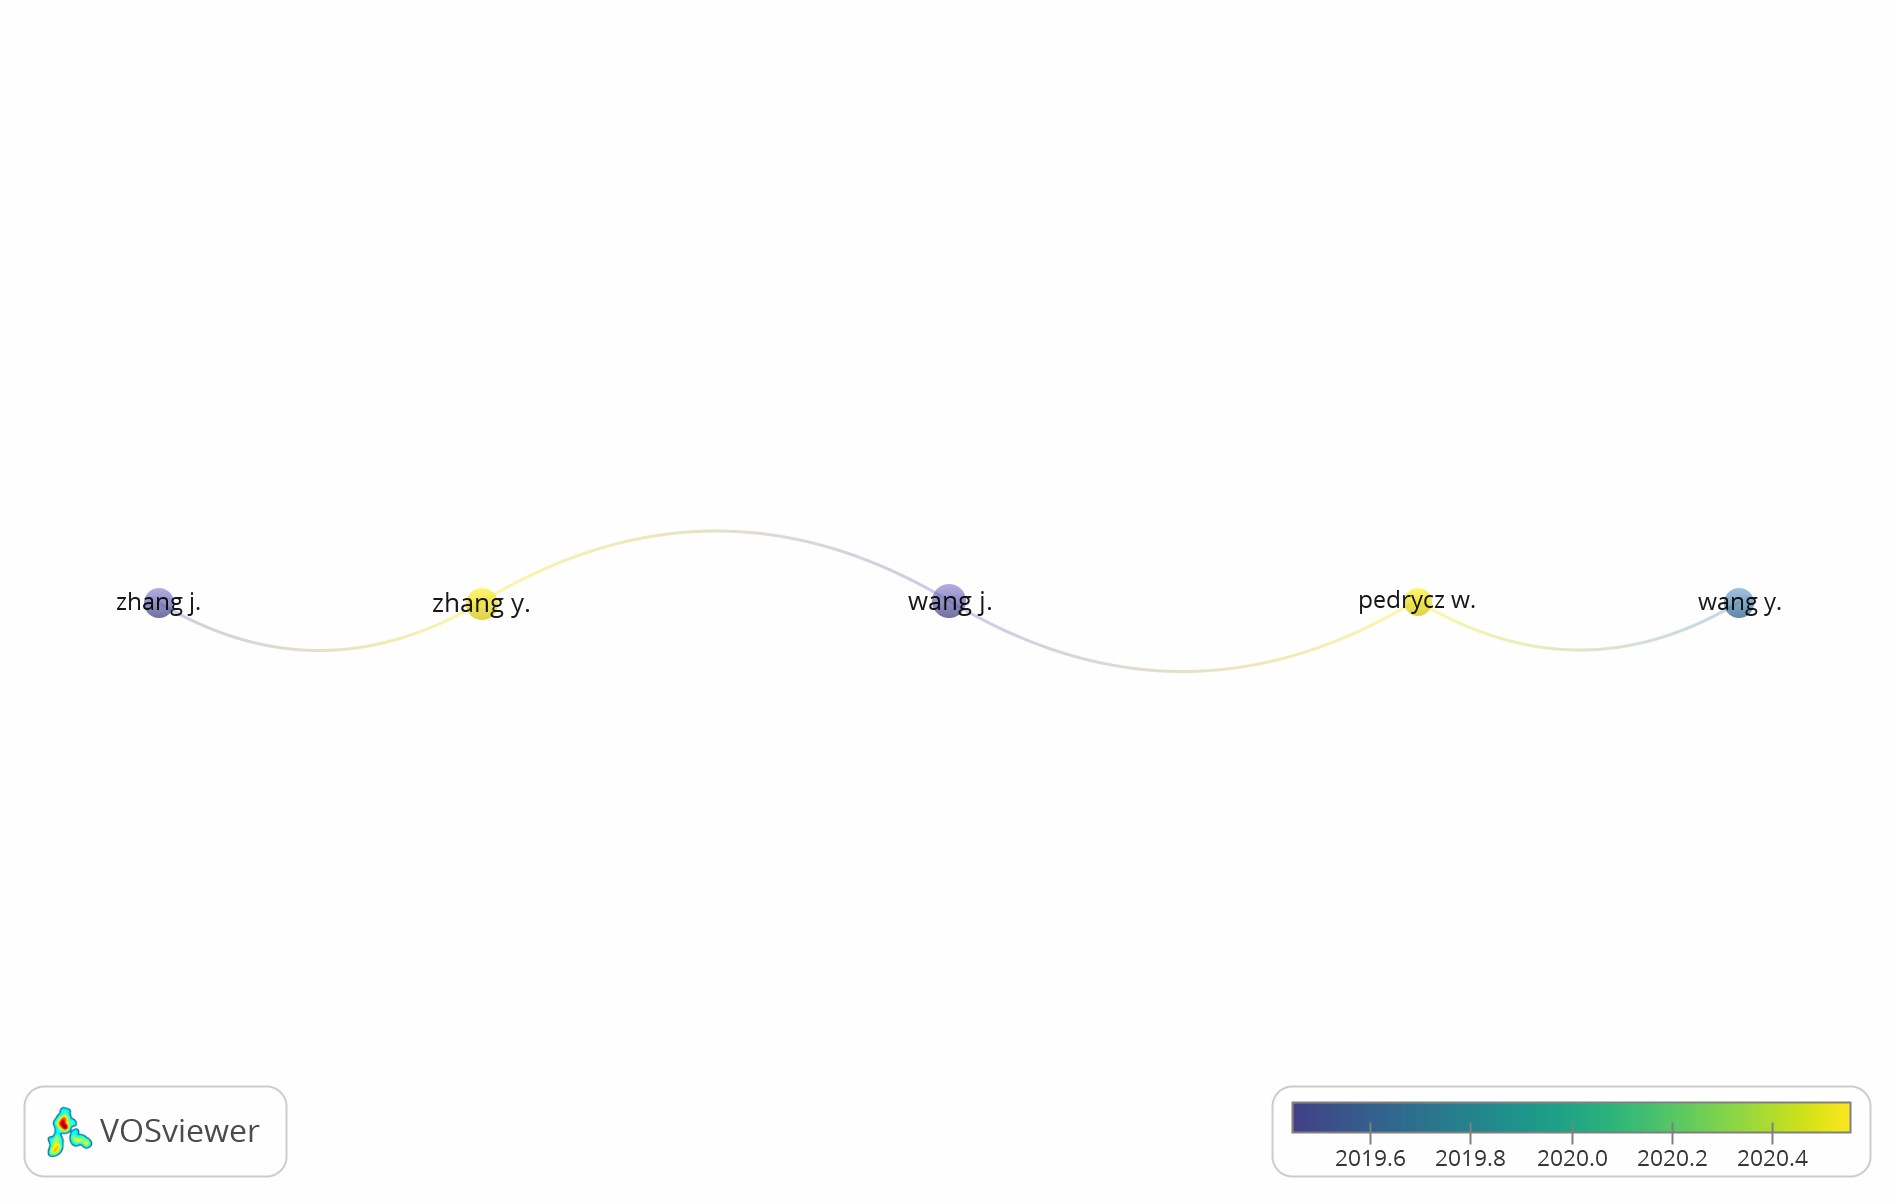
\includegraphics[width=0.8\linewidth]{Revisao/Figuras/Autores}
	
	\fonte{Elaboração própria a partir de dados da Scopus (2016 a 2022)}
\end{figure}

Em resposta à questão colocada anteriormente (\ref{questão:rev1}), foi utilizada a Figura \ref{fig:autores-relacao-entre-artigos-publicados} para visualizar de forma mais clara os autores que mais publicaram sobre o tema em análise. O gráfico apresenta um histograma que destaca os autores cujo número de publicações é maior que 4 durante o período de 2016 a 2022. Essa abordagem visa evitar a inclusão de todos os autores e destacar aqueles que tiveram uma contribuição significativa no campo, considerando o critério estabelecido de pelo menos 4 publicações. Dessa forma, é possível identificar os principais autores que se destacam nesse tópico específico, fornecendo uma visão geral da distribuição da produção científica entre os pesquisadores.


\begin{figure}[htpb!]
	\centering
	\caption{Mapa mundial da publicação de artigos em todo o mundo}
	\label{fig:mapa-mundi-artigos}
	\includegraphics[width=1\linewidth]{Revisao/Figuras/"mapa mundi artigos"}
	\vspace{0.2cm}
	
	\fonte{Elaboração própria a partir de dados da Scopus, Lens e Web of Sicence (2016 a 2022)}
\end{figure}

A pergunta de pesquisa \ref{questão:rev2} foi abordada por meio da análise da Figura \ref{fig:mapa-mundi-artigos}, que apresenta os países com maior número de publicações sobre o assunto em escala, ordenados de forma decrescente. Os principais países que se destacam nessa análise são os seguintes: China, com 119 publicações; Estados Unidos, com 67 publicações; Índia, com 57 publicações; Brasil, com 32 publicações; Espanha, com 28 publicações; Reino Unido, com 25 publicações; Austrália, com 24 publicações; Irã, com 18 publicações; Malásia, com 17 publicações; e Canadá, com 16 publicações.

É importante ressaltar que o mapa não exibe todos os países e seus respectivos números de publicações, mas destaca aqueles com maior produção nesse contexto específico. Essa análise ajuda a identificar os países com maior contribuição científica nessa área de estudo, fornecendo insights sobre os locais onde a pesquisa sobre séries temporais tem sido mais ativa.

\begin{figure}[htpb!]
	\centering
	\caption{Áreas de aplicação do tema}
	\label{fig:areas}
	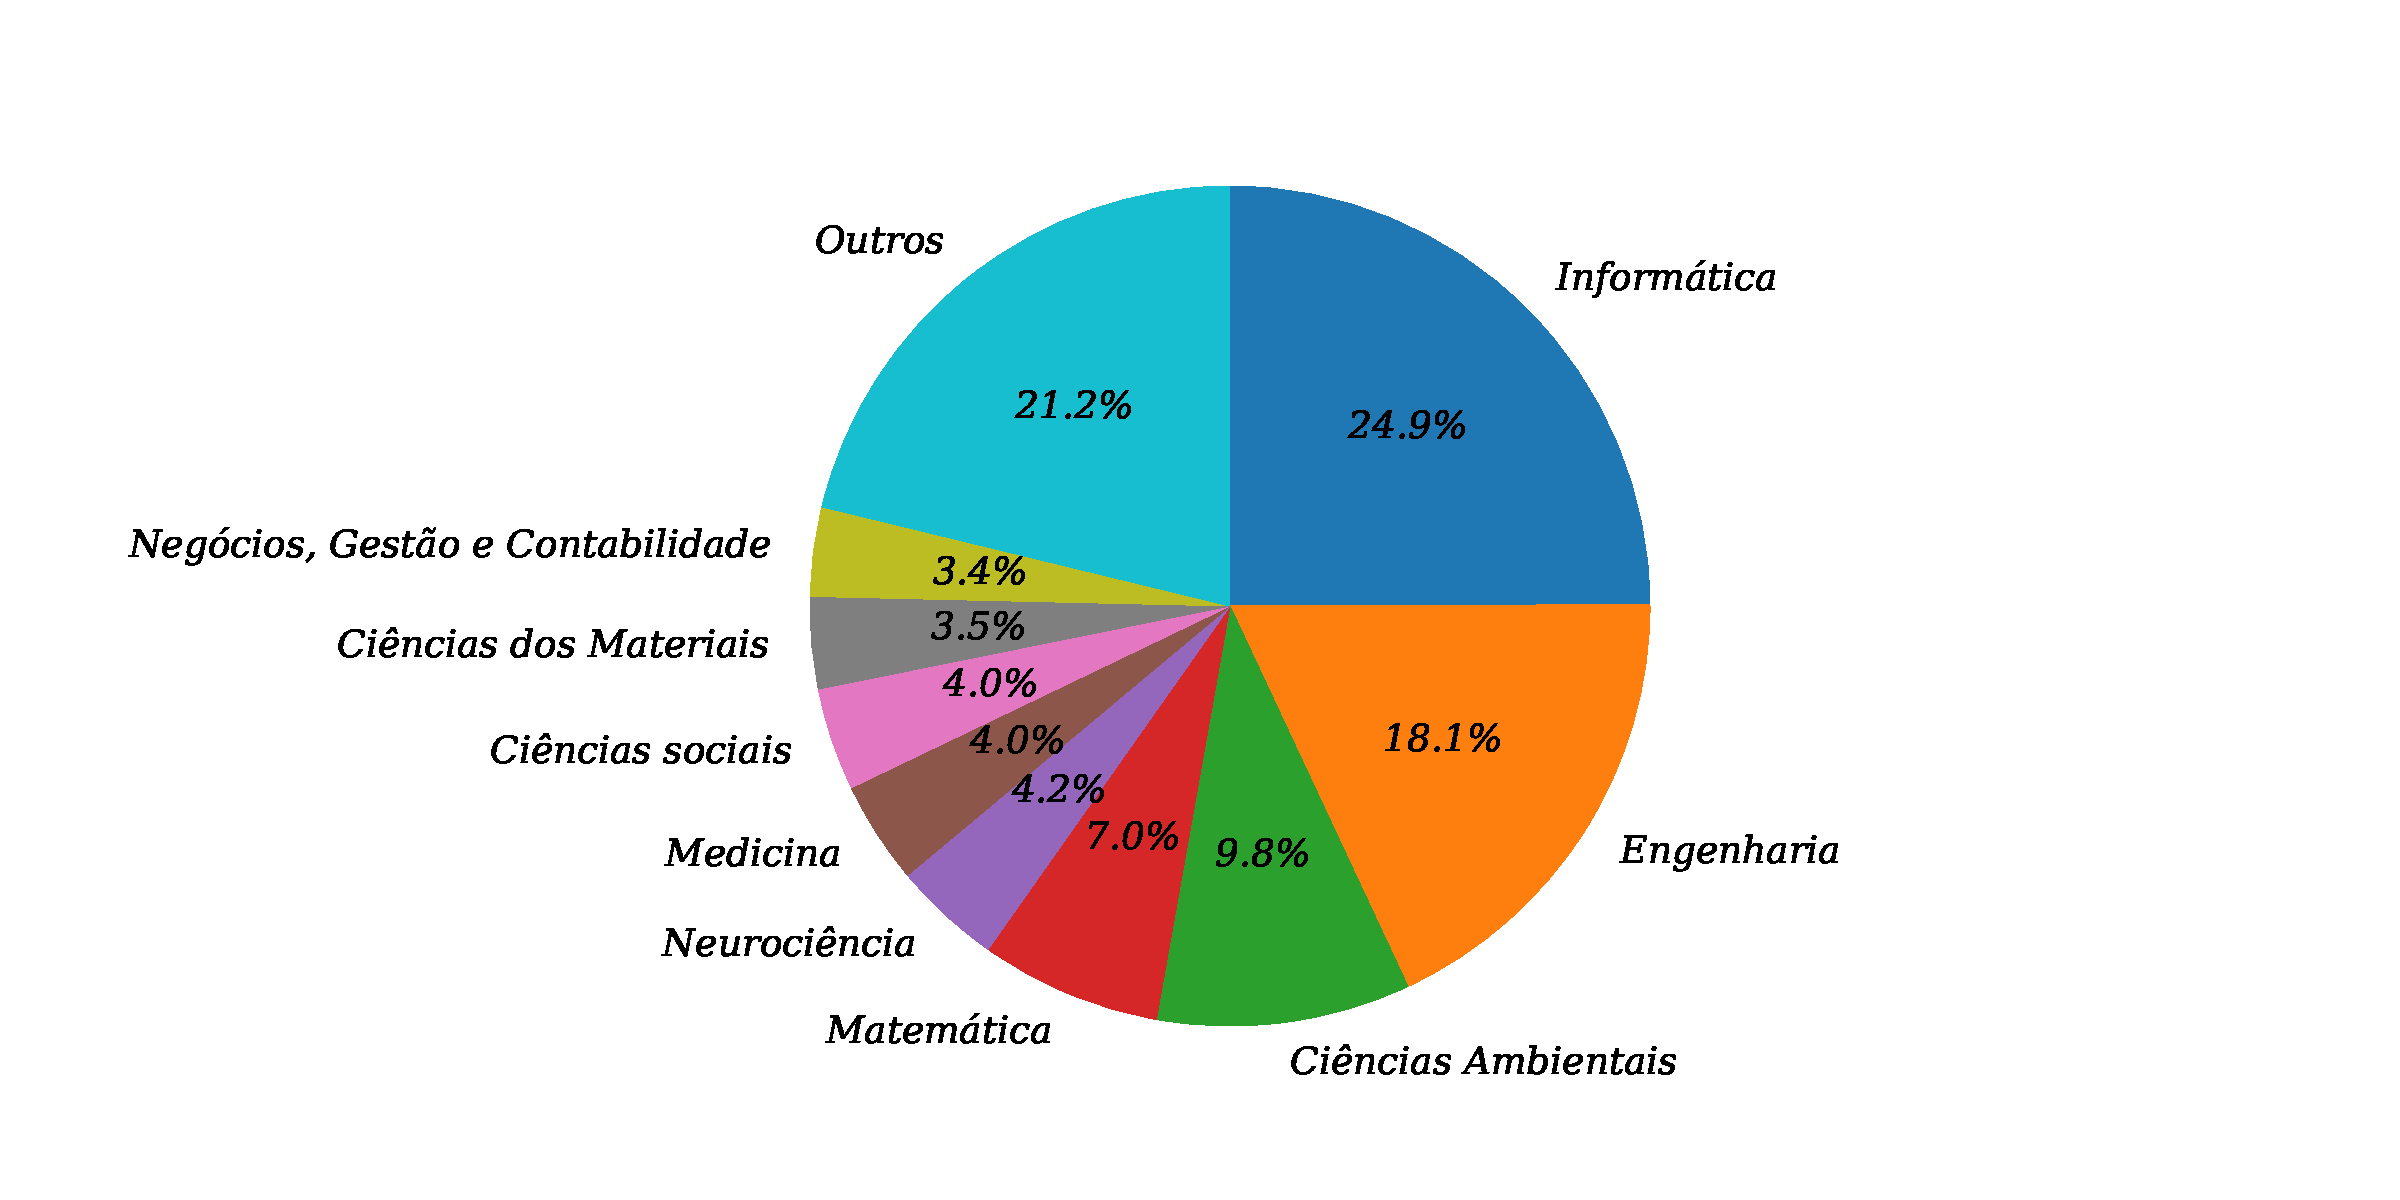
\includegraphics[width=0.9\linewidth]{Revisao/Figuras/areas}
	\vspace{0.2cm}
	
	\fonte{Elaboração própria a partir de dados da Scopus, Lens e Web of Sicence (2016 a 2022)}
\end{figure}


Para responder à pergunta de pesquisa \ref{questão:rev3}, foi criado um gráfico circular, apresentado na Figura \ref{fig:areas}, que ilustra as áreas com maior número de publicações durante o período analisado na revisão. A Tabela \ref{tb3} complementa o gráfico, fornecendo os valores específicos de cada área e a quantidade de publicações correspondente.

O gráfico circular oferece uma representação visual clara das áreas que se destacam em termos de produção científica no campo das séries temporais. Ao examinar a tabela, é possível identificar as áreas com maior número de publicações, permitindo uma compreensão aprofundada das principais áreas de conhecimento relacionadas ao tema. Essa análise contribui para uma melhor compreensão da distribuição de publicações e áreas de pesquisa ao longo do período estudado.

\begin{table}[!htb]
	\centering
	\caption{Áreas e seus valores respetivos de artigos em cada área.}\label{tb3}
	\begin{tabular}{@{}ll@{}}
		\toprule
		Informática                      & 240 \\ \midrule
		Engenharia                       & 174 \\
		Ciências Ambientais              & 94  \\
		Matemática                       & 67  \\
		Neurociência                     & 40  \\
		Medicina                         & 38  \\
		Ciências sociais                 & 38  \\
		Ciências dos Materias            & 34  \\
		Negócios, Gestão e Contabilidade & 33  \\
		Outros                           & 204 \\ \bottomrule
	\end{tabular}

	
	\fonte{Elaboração própria a partir de dados da Scopus, len e Web of Sicence (2016 a 2022)}
\end{table}




Na última pergunta de pesquisa, referente à \ref{questão:rev4}, foi realizada uma investigação dos artigos mais influentes na revisão. Esses artigos retratam alguns dos métodos utilizados por renomados autores \citeonline{Golyandina2020, Kumar2021, Xie2019, Lara-Benitez2021, Ahmad2018, CarvalhoJr.2019, Tan2021, Liu2019, Liu2021, Rossi2018, Soyer, Martinovic2020a, Ursu2016, Wang2016, Shih2019a, Moon2019, Chou2018, Bergmeir2018, Boroojeni2017, Chou2018a, Coelho2017, Du2020, Sadaei2019, Salgotra2020, Tyralis2017, Vlachas2020, Yang2019a, Shen2020, Sezer2020, Chen2018, Buyuksahin2019, Li2020, Kulshreshtha2020, Samanta2020, Xu2019, Graff2017, Taieb2016}. 

Esses artigos abordam diferentes métodos usados pelos autores para previsão de séries temporais e análise não-linear dessas previsões. Eles representam contribuições significativas para o avanço do conhecimento e aplicação prática das séries temporais, oferecendo insights valiosos sobre abordagens eficazes nesse campo. Ao incluir esses estudos influentes na análise, obtém-se uma visão abrangente dos métodos e técnicas mais relevantes na previsão de séries temporais.


No estudo conduzido por \citeonline{Xu2019}, um modelo híbrido foi proposto, combinando o modelo linear AR e LR com o modelo não-linear ARIMA e o modelo DBN. Essa abordagem permite capturar tanto os comportamentos lineares quanto os não-lineares de uma série temporal. Por outro lado, \citeonline{Li2020} comparou o desempenho de previsão da abordagem MAELS com outros modelos de aprendizado de máquina de última geração, como CNN, RNN, LSTM, ARIMA e SVM-VAR. As abordagens CNN, RNN e LSTM são capazes de lidar com dados multivariados de entrada e saída, enquanto o ARIMA utiliza informações passadas para prever o futuro com base em características como autocorrelação e médias móveis.

Dessa forma, por meio dessa revisão sistemática e análise de conteúdo, a pergunta de pesquisa formulada no início do capítulo foi respondida.

Além desses modelos mencionados, também será utilizada a versão atualizada do ARIMA nesta dissertação. Os modelos SARIMA e SARIMAX também serão comparados para determinar qual deles é o mais adequado. Além disso, serão empregados os modelos Light GBM e XGBoost. Quanto às métricas de erro, serão utilizadas MAE, MAPE e RMSE, que são amplamente adotadas na literatura. O coeficiente de determinação ($R^2$), mencionado na equação \eqref{eq2}, não é tão comumente utilizado para comparação de modelos de previsão futura.